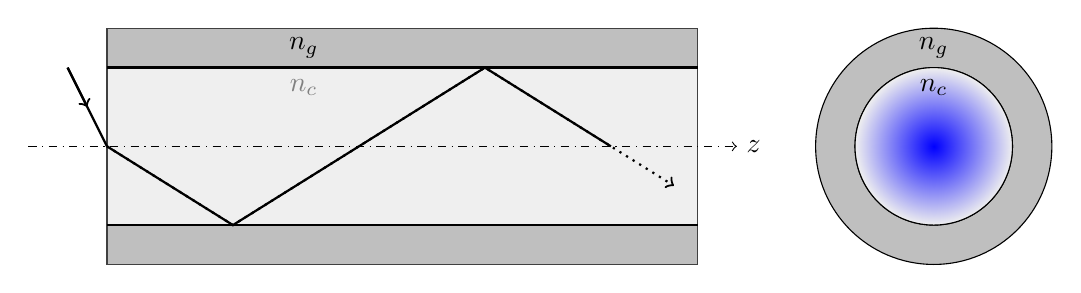
\begin{tikzpicture}

    % ==============
    % 1) LA FIBRE (vue de côté)
    % ==============
    % Enveloppe de la fibre
    \draw[color = gray!50!black, fill = lightgray] (0,-1.5) rectangle (7.5,1.5);
    % Coeur de la fibre
    \draw[color = gray!50!black, fill =  lightgray!25!white] (0,-1) rectangle (7.5,1);

    % Bords du coeur
    \draw[thick,black] (0,1) --++ (7.5,0);
    \draw[thick,black] (0,-1) --++ (7.5,0);

    % ==============
    % 2) AXE Z ET INDICES
    % ==============
    \draw[dashdotted,->] (-1,0) --++ (9,0) node[right]{$z$};
    
    % Indices
    \draw[gray]  (2.5, 0.75)  node{$n_c$};  % Coeur
    \draw[black] (2.5, 1.25)  node{$n_g$};  % Gaine

    % ==============
    % 3) RAYONS INCIDENTS ET TRAJET
    % ==============
    % Rayons d'entrée
    \draw[thick] (-0.5,1) --++ (0.5,-1);
    \draw[thick,->] (-0.5,1) --++ (0.25,-0.5);

    % Trajet "zigzag" dans la fibre (dotted = direction, thick = parois)
    \draw[dotted,thick,->] (0,0)
        --++ (1.6,-1)
        --++ (3.2,+2)
        --++ (2.4,-1.5);
    \draw[thick] (0,0)
        --++ (1.6,-1)
        --++ (3.2,+2)
        --++ (1.6,-1);

    % ==============
    % 4) SECTION DE LA FIBRE (vue en bout) - à droite
    % ==============
    % Gaine
    \draw[fill = lightgray, draw=black] (10.5,0) circle (1.5);

    % On réalise un "shading" radial pour le coeur : gaussienne ~ e^{-r^2/w_0^2}
    \begin{scope}
      % On découpe la zone du coeur de rayon 1
      \draw[fill = lightgray!25!white] (10.5,0) circle (1);
      % On applique un dégradé radial (du centre bleu vers les bords blancs)
      \shade[inner color=blue, outer color=lightgray!25!white] (10.5,0) circle (1);
    \end{scope}

    % Pour tracer le contour du coeur (si besoin)
    \draw[draw=black] (10.5,0) circle (1);

    % Labels pour n_c et n_g
    \draw (10.5,1.25) node{$n_g$};
    \draw (10.5,0.75) node{$n_c$};


\end{tikzpicture}

